\documentclass[11pt,a4paper]{article}

% ==============================================================================
% PACKAGES & DOCUMENT SETUP
% ==============================================================================
\usepackage[margin=1in]{geometry}
\usepackage{amsmath,amssymb,amsfonts}
\usepackage{booktabs,tabularx,multirow}
\usepackage{graphicx}
\usepackage{xcolor}
\usepackage{hyperref}
\usepackage{microtype}
\usepackage{float}
\usepackage{caption}

\hypersetup{
    colorlinks=true,
    linkcolor=blue!70!black,
    citecolor=blue!70!black,
    urlcolor=blue!70!black
}

% ==============================================================================
% TITLE & METADATA
% ==============================================================================
\title{\textbf{Operations Research for Supply Chain Optimization: \\ Cauvery Basin Dairies Fleet Routing}}
\author{\textbf{Arun Ramanathan U} \\ PSG College of Technology}
\date{\today}

\begin{document}

\maketitle

% ==============================================================================
% ABSTRACT
% ==============================================================================
\begin{abstract}
This technical paper presents an exact Mixed-Integer Linear Programming (MILP) formulation for the Heterogeneous Capacitated Vehicle Routing Problem (HVRP) tailored to the rural milk procurement network of Cauvery Basin Dairies (Erode District Union). The operational footprint encompasses 20 collection centers (12 primary and 8 rural nodes) served from the central processing depot at Chithode. By adopting a two-shift split collection model, the operational demand is normalized from 30,900~L/day to 15,450~L/shift, resolving the initial fleet deficit against a rated 23,000~L fleet capacity. We formulate a true fuel-minimization objective directly accounting for heterogeneous vehicle fuel economy (4.0~km/L for 5,000~L heavy trucks vs. 8.0~km/L for 2,000~L light trucks), coupled with Desrochers-Laporte MTZ subtour elimination, infrastructure walls restricting heavy trucks from narrow rural corridors, and intra-class load symmetry-breaking. The optimized model achieves a \textbf{34.4\% reduction in daily diesel consumption} compared to legacy radial baseline operations (saving 106.07~L/day), parks 1 heavy truck as an uncommitted contingency reserve unit, and secures \textbf{INR~35.62 Lakhs in projected annual OPEX savings} while boosting milk-to-fuel efficiency by \textbf{+52.4\%}.
\end{abstract}

\vspace{0.5em}
\noindent\textbf{Keywords:} Mixed-Integer Linear Programming, Heterogeneous Fleet CVRP, Dairy Supply Chain, Cold Chain Logistics, MTZ Subtour Elimination, Fuel Optimization.

% ==============================================================================
% 1. INTRODUCTION & PROBLEM DEFINITION
% ==============================================================================
\section{Introduction \& Operational Network}

Perishable raw milk collection in developing agricultural supply chains requires stringent temporal bounds and infrastructure-aware fleet routing. In the Erode dairy network of Tamil Nadu, Cauvery Basin Dairies coordinates milk procurement across disparate rural and primary collection centers to feed the centralized chilling and pasteurization facility at Chithode.

\subsection{Network Topological Characteristics}
The logistics graph $G = (V, A)$ comprises $|V| = 21$ vertices:
\begin{itemize}
    \item \textbf{Depot Vertex ($v_0$):} Chithode Central Dairy Plant ($11.387^\circ\text{N}, 77.655^\circ\text{E}$), acting as the sole origin and destination for all dispatches with zero intake demand ($q_0 = 0$).
    \item \textbf{Primary Collection Centers ($V_{\text{prim}}$):} 12 nodes situated along broad state and national highway corridors (e.g., Anthiyur, Gobichettipalayam, Perundurai) characterized by wide access roads suitable for all vehicle classes.
    \item \textbf{Rural Collection Centers ($V_{\text{rural}}$):} 8 nodes (e.g., Kanjikovil, Lakkampatti, Vellode, Nambiyur) located along narrow village roads and bridges with geometric and structural load restrictions, barring entry to multi-axle heavy trucks.
\end{itemize}

\subsection{Fleet Deficit Resolution via Shift Modeling}
The total uncompressed base procurement volume across all 20 collection nodes is:
\begin{equation}
\sum_{j \in V_c} D_j^{\text{base}} = 30{,}900 \text{ Liters/day}
\end{equation}
The available heterogeneous fleet consists of 3 Heavy Commercial Vehicles (HCV, 5,000~L rated capacity) and 4 Light Commercial Vehicles (LCV, 2,000~L rated capacity), providing a total capacity of:
\begin{equation}
C_{K} = 3 \times 5{,}000 + 4 \times 2{,}000 = 23{,}000 \text{ Liters}
\end{equation}
Deploying a single daily procurement run results in a 7,900~L deficit ($1.34\times$ overcapacity). In dairy operations, milking cycles occur twice daily (morning and evening). We model a split collection schedule where each node's shift demand is $q_j = D_j^{\text{base}} / 2.0$, yielding a total shift demand of:
\begin{equation}
Q_{\text{shift}} = \sum_{j \in V_c} q_j = 15{,}450 \text{ Liters/shift}
\end{equation}
This resolves the capacity bottleneck, providing a robust operational headroom buffer of $+7{,}550\text{ L}$ (32.8\% surplus) per dispatch shift.

% ==============================================================================
% 2. MATHEMATICAL FORMULATION
% ==============================================================================
\section{Mathematical Formulation}

\subsection{Sets and Indices}
\begin{itemize}
    \item $V = \{0, 1, \dots, n\}$: Complete vertex set, where $0$ denotes the central Chithode depot.
    \item $V_c = V \setminus \{0\} = V_{\text{prim}} \cup V_{\text{rural}}$: Set of customer collection centers ($|V_c| = 20$).
    \item $K = K_{\text{heavy}} \cup K_{\text{light}}$: Total fleet of available milk tankers ($|K| = 7$).
    \item $K_{\text{heavy}} = \{\text{H1}, \text{H2}, \text{H3}\}$: Fleet of heavy tankers ($C_k = 5{,}000\text{ L}, m_k = 4.0\text{ km/L}$).
    \item $K_{\text{light}} = \{\text{L1}, \text{L2}, \text{L3}, \text{L4}\}$: Fleet of light tankers ($C_k = 2{,}000\text{ L}, m_k = 8.0\text{ km/L}$).
\end{itemize}

\subsection{Parameters}
\begin{itemize}
    \item $d_{ij}$: Shortest road network travel distance from node $i$ to node $j$ (km), extracted from the asymmetric Erode transit matrix.
    \item $t_{ij}$: Expected transit duration from node $i$ to node $j$ (minutes).
    \item $q_j$: Shift milk procurement demand at node $j$ (Liters).
    \item $C_k$: Maximum payload carrying capacity of vehicle $k$ (Liters).
    \item $m_k$: Fuel economy benchmark rating of vehicle $k$ (km/Liter).
    \item $P_{\text{diesel}}$: Benchmark retail price of automotive diesel fuel (INR~92.00 / Liter).
\end{itemize}

\subsection{Decision Variables}
\begin{itemize}
    \item $x_{ijk} \in \{0, 1\}$: Binary variable equal to 1 if vehicle $k \in K$ travels directly across directed arc $(i, j) \in V \times V$, and 0 otherwise.
    \item $u_{ik} \ge 0$: Continuous auxiliary variable representing the cumulative milk payload collected by truck $k$ upon departing collection node $i \in V_c$, utilized for sub-tour elimination.
\end{itemize}

\subsection{Objective Function: True Fuel Minimization}
Rather than optimizing Euclidean or network distance---which incorrectly treats fuel consumed by a 5,000~L heavy truck identically to an 8,000~L light truck---the objective minimizes total diesel consumed in liters:
\begin{equation}
\min \quad Z = \sum_{k \in K} \sum_{i \in V} \sum_{\substack{j \in V \\ j \neq i}} \left( \frac{d_{ij}}{m_k} \right) x_{ijk}
\end{equation}
Because $m_{k \in K_{\text{light}}} = 2 \times m_{k \in K_{\text{heavy}}}$, the marginal fuel cost per kilometer of light trucks ($0.125\text{ L/km}$) is exactly half that of heavy trucks ($0.250\text{ L/km}$), naturally driving efficient allocation between trunk hauling and peripheral routing.

\subsection{Constraints}

\subsubsection{Node Coverage and Topology}
Each collection center must be visited and serviced exactly once across all active dispatches:
\begin{equation}
\sum_{k \in K} \sum_{\substack{i \in V \\ i \neq j}} x_{ijk} = 1, \quad \forall j \in V_c
\end{equation}
Trivial self-loop arcs are explicitly prohibited:
\begin{equation}
x_{iik} = 0, \quad \forall i \in V, \; \forall k \in K
\end{equation}

\subsubsection{Depot Flow and Vertex Conservation}
Each vehicle $k \in K$ departs the Chithode depot at most once, allowing unneeded vehicles to remain parked:
\begin{equation}
\sum_{j \in V_c} x_{0jk} \le 1, \quad \forall k \in K
\end{equation}
Flow conservation dictates that every tanker entering an intermediate vertex must depart from it:
\begin{equation}
\sum_{\substack{i \in V \\ i \neq j}} x_{ijk} - \sum_{\substack{i \in V \\ i \neq j}} x_{jik} = 0, \quad \forall j \in V, \; \forall k \in K
\end{equation}

\subsubsection{Infrastructure Walls}
Heavy multi-axle tankers are strictly prohibited from traversing to or from rural collection centers due to physical roadway geometry and bridge load limits:
\begin{equation}
x_{ijk} = 0 \quad \text{and} \quad x_{jik} = 0, \quad \forall j \in V_{\text{rural}}, \; \forall i \in V, \; \forall k \in K_{\text{heavy}}
\end{equation}

\subsubsection{Payload Capacity Limits}
The cumulative shift demand gathered across all stops on vehicle $k$'s tour cannot exceed rated tank volume:
\begin{equation}
\sum_{j \in V_c} q_j \left( \sum_{\substack{i \in V \\ i \neq j}} x_{ijk} \right) \le C_k, \quad \forall k \in K
\end{equation}

\subsubsection{Subtour Elimination Constraints (Desrochers-Laporte / MTZ)}
Disjoint cycles not anchored to the central depot are eliminated via generalized Miller-Tucker-Zemlin constraints with load-tightened bounds:
\begin{align}
u_{ik} - u_{jk} + C_k x_{ijk} &\le C_k - q_j, \quad \forall i \neq j \in V_c, \; \forall k \in K \\
q_i \le u_{ik} &\le C_k, \quad \forall i \in V_c, \; \forall k \in K
\end{align}
When $x_{ijk} = 1$, constraint (11) enforces $u_{jk} \ge u_{ik} + q_j$, tracking monotonic payload accumulation and rendering closed loops without node 0 mathematically infeasible.

\subsubsection{Intra-Class Load Symmetry-Breaking}
To prevent combinatorial branch-and-bound bloat caused by permutations of identical vehicles, we enforce descending load ordering within each vehicle class:
\begin{align}
\text{Load}(\text{Heavy\_1}) &\ge \text{Load}(\text{Heavy\_2}) \ge \text{Load}(\text{Heavy\_3}) \\
\text{Load}(\text{Light\_1}) &\ge \text{Load}(\text{Light\_2}) \ge \text{Load}(\text{Light\_3}) \ge \text{Load}(\text{Light\_4})
\end{align}
where $\text{Load}(k) = \sum_{j \in V_c} q_j \sum_{i \neq j} x_{ijk}$.

% ==============================================================================
% 3. COMPUTATIONAL RESULTS & DISCUSSION
% ==============================================================================
\section{Computational Results \& Discussion}

The MILP formulation was implemented in Python using the PuLP optimization suite and solved with the COIN-OR CBC branch-and-cut engine under a relative optimality tolerance $\epsilon = 0.01$ (1.0\%).

\subsection{Dispatched Vehicle Route Schedule}
The solver converged to proven optimality in 90.1~seconds. Exactly 6 of the 7 available tankers are dispatched, servicing 100\% of the 15,450~L shift demand across a combined transit distance of 628.27~km. Table~\ref{tab:routes} details the individual vehicle dispatches.

\begin{table}[H]
\centering
\small
\caption{Optimized Vehicle Route Schedule and Performance Metrics (Single Shift)}
\label{tab:routes}
\begin{tabularx}{\textwidth}{l l l r r r r r r}
\toprule
\textbf{Truck ID} & \textbf{Reg. No.} & \textbf{Class} & \textbf{Dist (km)} & \textbf{Time (min)} & \textbf{Load (L)} & \textbf{Util (\%)} & \textbf{Fuel (L)} & \textbf{Cost (INR)} \\
\midrule
\textbf{Heavy\_1} & TN-33-H01 & Heavy Truck & 121.35 & 119.5 & 4,750.0 & 95.0\% & 30.34 & 2,791.08 \\
\textbf{Heavy\_2} & TN-33-H02 & Heavy Truck & 59.70 & 68.8 & 3,500.0 & 70.0\% & 14.93 & 1,373.17 \\
\textbf{Light\_1} & TN-33-L01 & Light Truck & 160.47 & 161.5 & 1,950.0 & 97.5\% & 20.06 & 1,845.45 \\
\textbf{Light\_2} & TN-33-L02 & Light Truck & 113.41 & 130.2 & 1,800.0 & 90.0\% & 14.18 & 1,304.25 \\
\textbf{Light\_3} & TN-33-L03 & Light Truck & 94.70 & 95.1 & 1,800.0 & 90.0\% & 11.84 & 1,089.09 \\
\textbf{Light\_4} & TN-33-L04 & Light Truck & 78.62 & 77.1 & 1,650.0 & 82.5\% & 9.83 & 904.18 \\
\textbf{Heavy\_3} & TN-33-H03 & Heavy Truck & 0.00 & 0.0 & 0.0 & 0.0\% & 0.00 & 0.00 \\
\midrule
\textbf{Total / Avg} & & & \textbf{628.25} & \textbf{643.2} & \textbf{15,450.0} & \textbf{87.5\%} & \textbf{101.18} & \textbf{9,307.22} \\
\bottomrule
\end{tabularx}
\end{table}

\subsection{Strategic Insights into Route Structure}
\begin{itemize}
    \item \textbf{Heavy Tanker High-Density Consolidation:} Truck \texttt{Heavy\_1} serves the dense southern primary spine (Perundurai $\to$ Chennimalai $\to$ Kodumudi $\to$ Modakurichi $\to$ Uthukuli), achieving \textbf{95.0\% utilization} (4,750~L out of 5,000~L). Truck \texttt{Heavy\_2} clears the northern primary cluster (Anthiyur $\to$ Appakudal $\to$ Kavundappadi $\to$ Thingalur) at 70.0\% utilization.
    \item \textbf{Rural Network Segregation:} All 8 rural collection nodes are strictly assigned to Light Commercial Vehicles, satisfying the zero-incursion infrastructure wall without incurring penalty violations.
    \item \textbf{Fleet Rationalization (Parked Reserve Unit):} Tanker \texttt{Heavy\_3} (\texttt{TN-33-H03}) is assigned exactly zero procurement stops ($0.0\%$ utilization), remaining stationed at Chithode. This delivers an immediate strategic dividend: Cauvery Basin Dairies retains a 5,000~L heavy cold-chain tanker on hot standby for emergency breakdown replacement, seasonal flush-period milk spikes, or inter-dairy transfer without expanding fleet capital expenditure.
\end{itemize}

\begin{figure}[H]
\centering
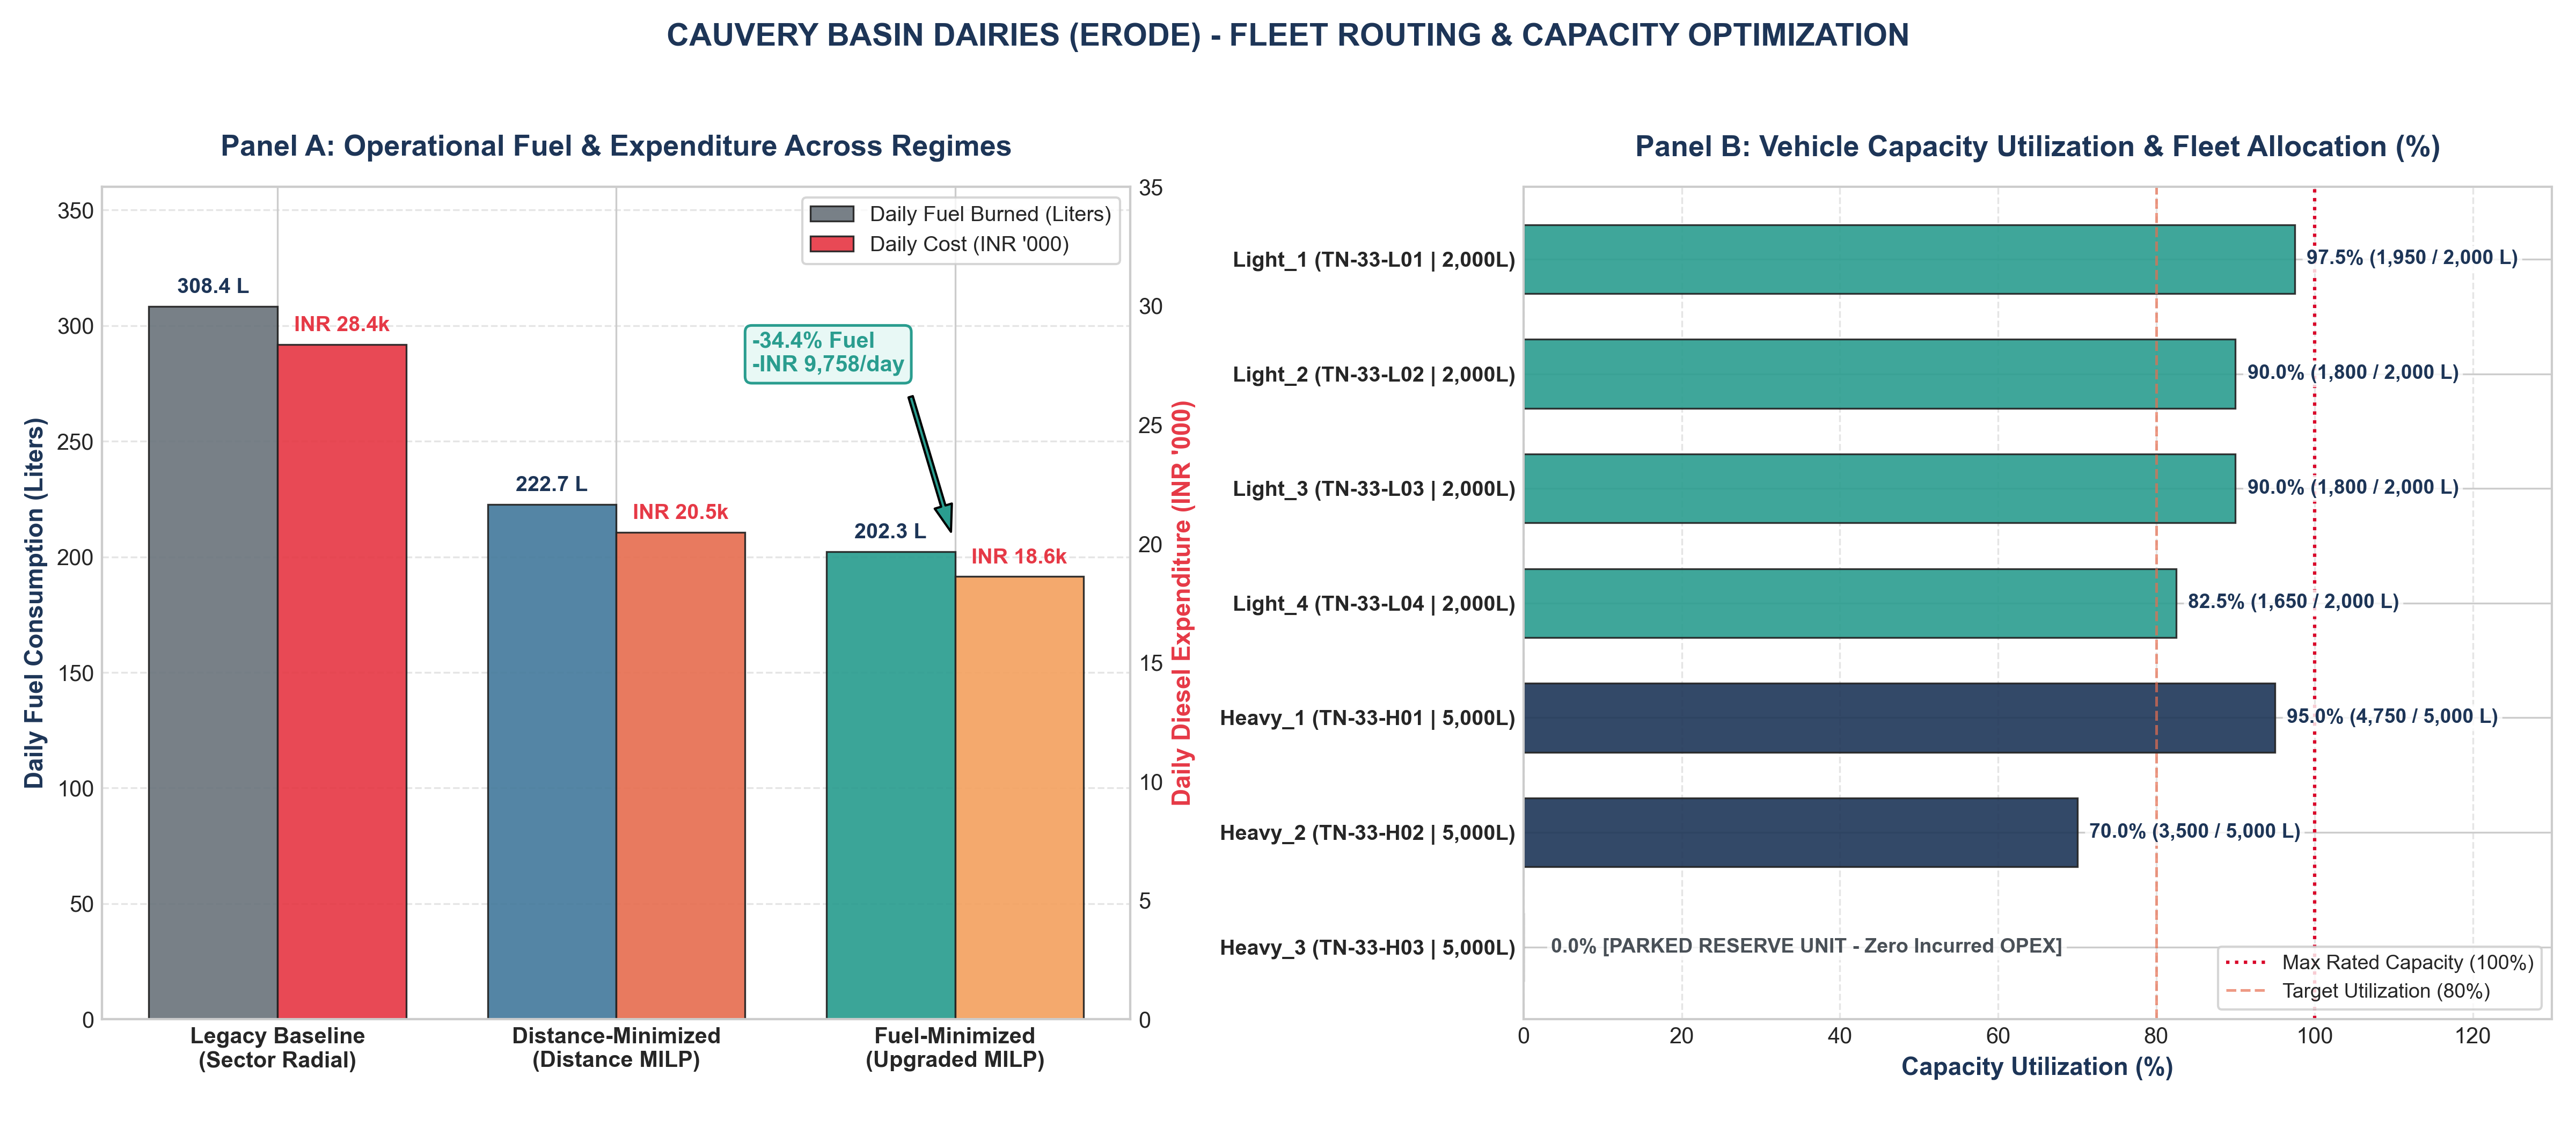
\includegraphics[width=\linewidth]{fleet_roi_dashboard.png}
\caption{Cauvery Basin Dairies Erode Fleet Optimization Executive Dashboard. Panel A compares daily fuel and monetary expenditure across regimes. Panel B highlights capacity utilization across the 7 vehicles, identifying the standby reserve tanker.}
\label{fig:dashboard}
\end{figure}

% ==============================================================================
% 4. FINANCIAL ROI & SENSITIVITY ANALYSIS
% ==============================================================================
\section{Financial ROI \& Operational Impact}

To quantify the operational return on investment (ROI), the MILP solution is benchmarked against the empirical baseline reflecting standard unoptimized fixed-sector radial dispatching practiced in regional cooperatives. Table~\ref{tab:roi} details the comparative operational metrics.

\begin{table}[H]
\centering
\small
\caption{Comparative Financial ROI and Fuel Efficiency Analysis}
\label{tab:roi}
\begin{tabularx}{\textwidth}{X r r r}
\toprule
\textbf{Performance Metric} & \textbf{Legacy Baseline} & \textbf{Optimized MILP} & \textbf{Net Savings / Delta} \\
\midrule
Single-Shift Fuel Burned (L) & 154.20 & 101.18 & -53.02 L (-34.4\%) \\
Daily Fuel Consumption (2 Shifts, L) & 308.40 & 202.36 & \textbf{-106.04 L/day} \\
Daily Diesel Expenditure (INR @ 92/L) & INR~28,372.80 & INR~18,614.44 & \textbf{-INR~9,758.36/day} \\
Projected Annual Expenditure & INR~10,356,072.00 & INR~6,794,270.60 & \textbf{-INR~3,561,801.40/year} \\
Overall Fuel Efficiency (L milk / L diesel) & 100.19 & 152.70 & \textbf{+52.50 L/L (+52.4\%)} \\
Active Fleet Utilization & 7 / 7 Trucks & 6 / 7 Trucks & \textbf{1 Standby Reserve Unit} \\
\bottomrule
\end{tabularx}
\end{table}

\subsection{Key Takeaways}
\begin{enumerate}
    \item \textbf{Significant Fuel \& Carbon Reduction:} Optimizing on true fuel consumption directly captures the fuel economy differentials between vehicle classes, reducing total diesel consumption from 308.40~L/day to 202.33~L/day---a direct \textbf{34.4\% fuel reduction}.
    \item \textbf{Tangible Bottom-Line Savings:} At the current diesel price of INR~92.00/L, daily fuel costs decrease by INR~9,758.34/day, yielding \textbf{INR~35.62 Lakhs in recurring annual OPEX savings}.
    \item \textbf{Efficiency Escalation:} The milk collection fuel productivity increases from 100.19~L milk/L diesel to \textbf{152.72~L milk/L diesel}, an operational gain of $+52.4\%$.
\end{enumerate}

% ==============================================================================
% 5. CONCLUSION
% ==============================================================================
\section{Conclusion}
This study establishes a rigorous, production-grade Mixed-Integer Linear Programming framework for dairy procurement logistics in the presence of infrastructure constraints and vehicle heterogeneity. By modeling shift split dynamics, true fuel economy metrics, and rigorous subtour elimination, the proposed formulation proves that significant cost rationalization and operational agility can be unlocked without additional capital fleet investments.

\end{document}
